This section details the software components within the Client and Cloud tiers, defining their specific responsibilities and interactions.

\subsection{Hybrid Client Components}
\begin{itemize}
    \item \textbf{Native Bridge (Capacitor):} The architectural boundary between the web code and the native OS. It exposes a unified API to access hardware features. It ensures that the \textbf{Geolocation} and \textbf{Accelerometer} continue to operate reliably even when the application is in the background, bridging the gap between the web runtime and the device hardware.
    
    \item \textbf{Sensor Controller \& Filter:} Responsible for logic related to data acquisition.
    \begin{itemize}
        \item It interfaces with the \textbf{Native Bridge} to subscribe to GPS and Accelerometer streams.
        \item It implements a \textbf{Kalman Filter} to smooth raw GPS coordinates.
        \item It analyzes accelerometer data to detect vertical shocks (road surface irregularities like potholes) and buffers this data locally during activity recording.
    \end{itemize}
    
    \item \textbf{Local Persistence Manager:} Implements the "Offline-First" capability. It uses an embedded database (e.g., SQLite via Capacitor plugin) to store activity traces and pending reports when the network is unavailable. It includes a \textbf{Sync Engine} that monitors network reachability and uploads buffered data to the cloud once connectivity is restored.
    
    \item \textbf{BaaS Client SDK:} The abstraction layer provided by the BaaS platform. It manages the persistent WebSocket connection for real-time updates, handles secure API calls to the database, and automatically refreshes authentication tokens.
    
    \item \textbf{Map \& UI Controller:} Manages the visualization of map tiles and path geometries. It handles user inputs (forms, search queries) and renders the visual feedback for the navigation system.
\end{itemize}

\subsection{Managed Cloud Components (BaaS)}
\begin{itemize}
    \item \textbf{Auth Service (Identity Provider):} Manages user lifecycles (sign-up, login, password recovery). It integrates with third-party OAuth providers (e.g., Google, Facebook) and issues secure JWTs containing user roles and IDs.
    
    \item \textbf{Spatial Database (PostgreSQL + PostGIS):} The central data repository. It is an active component that:
    \begin{itemize}
        \item Enforces \textbf{RLS Policies} to secure data access.
        \item Executes complex \textbf{Spatial Queries} (e.g., \texttt{ST\_DWithin}, \texttt{ST\_Intersects}) natively, allowing clients to efficiently retrieve paths within a specific viewport.
        \item Triggers database events (Webhooks) to activate Edge Functions upon data changes.
    \end{itemize}
    
    \item \textbf{Object Storage:} A specialized file storage system for large binary assets, such as user profile pictures or images attached to path reports.
\end{itemize}

\subsection{Backend Logic: Database Functions and Edge Functions}
The system architecture differentiates between \textbf{Database Functions} (RPC and Triggers), which handle data-intensive geospatial operations, and \textbf{Edge Functions}, which manage external requests and orchestration.

\subsubsection{Database Functions (RPC and Triggers)}
The following functions are implemented within the PostgreSQL engine to leverage PostGIS spatial indexing and ensure data integrity:

\begin{itemize}
    \item \texttt{check\_path\_similarity}
    \begin{itemize}
        \item \textbf{Type:} Remote Procedure Call (RPC).
        \item \textbf{Parameters:} \texttt{new\_geom\_wkt} (Text), \texttt{tolerance\_meters} (Default: 50), \texttt{length\_tolerance\_pct} (Default: 0.2).
        \item \textbf{Responsibility:} Implements the \textbf{Geometric Integrity Control}. It compares a newly recorded or drawn track against the existing database using Fréchet distance and length heuristics. It returns a table of similar paths, enabling the system to prevent duplicates or suggest merging activities into existing community paths.
    \end{itemize}

    \item \texttt{get\_path\_community\_usage}
    \begin{itemize}
        \item \textbf{Type:} Security Function (Definer).
        \item \textbf{Responsibility:} Analyzes the usage of a specific path by checking the number of activities linked to it by users other than the owner. This is a critical \textbf{Data Protection} mechanism: if a path is actively used by the community, the original creator is restricted from deleting it or switching it to private mode.
    \end{itemize}

    \item \texttt{search\_best\_paths\_rpc}
    \begin{itemize}
        \item \textbf{Type:} Geospatial RPC.
        \item \textbf{Responsibility:} Core of the \textbf{Search Algorithm}. It identifies candidate paths within a spatial buffer between the origin and destination coordinates. It calculates a match score based on how well the path's geometry aligns with the requested route, returning a ranked list of the best available options.
    \end{itemize}

    \item \texttt{handle\_new\_user}
    \begin{itemize}
        \item \textbf{Type:} Auth Trigger.
        \item \textbf{Responsibility:} Automatically manages the creation of user profiles in the public schema upon a successful authentication event, ensuring consistent user management.
    \end{itemize}
\end{itemize}

\subsubsection{Edge Functions}
These are serverless, stateless functions used for client-side interaction and external API orchestration:

\begin{itemize}
    \item \texttt{func\_path\_search}
    \begin{itemize}
        \item \textbf{Trigger:} Direct Client Request.
        \item \textbf{Responsibility:} Acts as an \textbf{API Gateway} for the path search feature. It receives coordinates from the client, validates the request, and invokes the internal \texttt{search\_best\_paths\_rpc}. This separation allows for future implementation of multi-source data enrichment (e.g., combining database results with external routing engine data) before returning the ranked results to the UI.
    \end{itemize}
\end{itemize}

\begin{figure}[H]
    \centering
    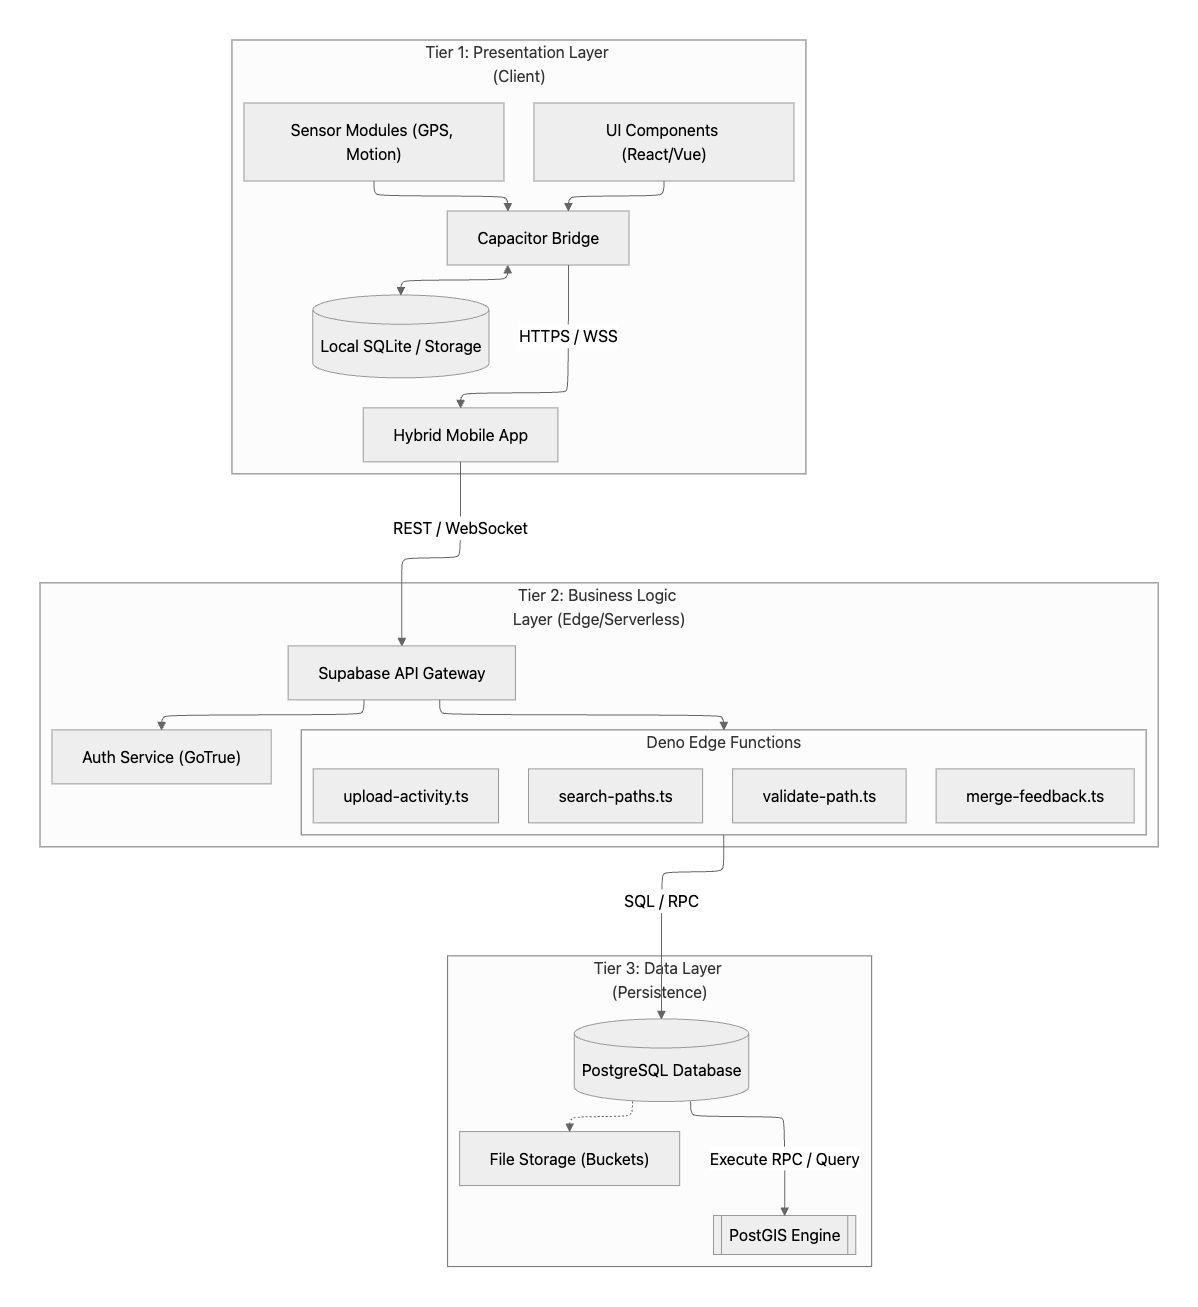
\includegraphics[width=\textwidth]{Images/system_architecture.jpg}
    \caption{Architectural Overview}
    \label{fig:arch_overview}
\end{figure}